\documentclass[11pt]{article}
\usepackage[margin=1.1in]{geometry}
\usepackage{amsmath,amssymb}
\usepackage{graphicx}
\usepackage{booktabs}
\usepackage{multirow}
\usepackage{microtype}
\usepackage[hidelinks]{hyperref}
\usepackage{xcolor}

\newcommand{\reg}{\textsc{Registry}}
\newcommand{\rrho}{\rho}

\title{One Registry, Several Jobs: An Empirical Map of Online Co-activation
Assemblies in Small Transformers---Emergence, the Limits of Pattern Completion,
and Free Internal-Fault Monitoring}

\author{Anonymous\thanks{Author information withheld in this draft. Code and all
raw results are included in the accompanying archive. Substantial portions of
the experimental engineering and drafting were carried out with the assistance
of an AI system under human direction; all claims were checked against logged
experimental outputs.}}
\date{August 2026}

\begin{document}
\maketitle

\begin{abstract}
We empirically map a single, biologically inspired primitive across every job it
has been proposed to do. The primitive is a \emph{co-activation assembly
registry}: during ordinary training, the set of hidden units whose activation
exceeds half of the per-position maximum is registered online into a bounded
number of groups by Jaccard overlap, together with each group's typical
activation values. Across more than twenty experiments on small Transformers
(34--112k parameters) and one 82M pretrained language model, all on 2 CPU
cores, we find a sharply structured answer to ``what is this mechanism actually
good for?''
(1)~\emph{Emergence is real}: on a synthetic language with latent word classes,
class-level assemblies form during training and are captured online---exactly 8
groups for 8 planted classes, 100\% class purity, zero cross-class merges,
replicated over 3 seeds; on real text, assemblies also form but the state
inventory is 340--450 groups, not 8, and registry capacity must match it.
(2)~\emph{Completion is causal but bounded}: injecting a matched group's missing
units repairs damage inflicted at the completion site (78\% of corruption loss
recovered), with wrong-content placebos strictly harmful in every experiment;
yet completion cannot rescue naturally under-trained tokens---the tokens broken
enough to need repair are exactly those whose group can no longer be retrieved
reliably (52\% correct at 11 training occurrences, against 99\% at 77)---and cannot induce
compositional generalization, because the network's set-stable cores organize by
\emph{execution progress} rather than by composable semantics. On real text the
repair effect dilutes from 78\% to 7\% as the group inventory grows.
(3)~\emph{The same registry, read instead of written, is a free internal-fault
sentinel}: two readings---which units are lit, and whether lit units have
typical values---detect four families of internal faults (unit zeroing, Gaussian
noise, stuck-at-zero units, quantization distortion) at AUC $\ge 0.95$ for
moderate severity, beat a perplexity baseline exactly where output-level
monitoring is weakest (0.955 vs.\ 0.732 at 30\% unit damage), and localize the
faulty layer through an upstream-silence signature (upstream detector at
chance-level 0.500 when the fault is downstream). (4)~\emph{The sentinel transfers to a real pretrained LM}: on distilgpt2 (82M
parameters), unit-level faults are detected at AUC 0.94--1.00 and the
upstream-silence localization signature is, if anything, cleaner than in the
toy setting (downstream echo 0.53; upstream exactly 0.500); value-level faults
(noise, quantization) degrade at this scale and are flagged as an open
weakness. Critically, a registry built \emph{during} actual continued
pretraining (400 gradient steps, domain loss 4.08$\rightarrow$3.05) matches a
post-hoc profiling pass (drop-fault AUC 0.93 vs.\ 0.92) and even repairs the
quantization blind spot (value channel 0.97)---so the ``free by-product of
training'' property holds under real weight updates, not just in code-path
form. A stale archive from before the continued pretraining dissociates by
channel: co-activation \emph{topology} survives training drift (AUC
0.92--1.00) while typical \emph{values} do not (0.55--0.59)---assembly
structure is more persistent than activation magnitudes. We position all this
against existing activation-monitoring work (Mahalanobis, activation-pattern,
and fault-fingerprint monitors): the individual capabilities are not
unprecedented; what is new is that they come from a streaming structure built
for free during training, with no post-hoc profiling and no fault-injection
calibration, and that detection and repair share one mechanism.
(5)~\emph{Deployment exposes what the AUCs hide}: judged one document at a
time, alarm rate does not track harm (freezing 30\% of units costs twice the
loss of deleting 30\% of active ones and is caught half as often), damage
outside the assemblies is structurally invisible (alarm rate equal to the
healthy baseline to the digit, though member units carry $13\times$ the
damage), and a healthy model reading out-of-domain text false-alarms at
95\%---which a domain-diverse archive plus within-document judging reduces to
0\% with no loss of detection or localization. Once an alarm does fire,
86--100\% of alarms name the correct layer.
(6)~\emph{The failure is the carrier, not the idea}: standard activation
patching---never run in the experiments above, which were all additive---shows
that replacing a deficient state with a real \emph{same-context} state recovers
98\% of the achievable benefit, while a state of the same class transported from
another context is catastrophic ($+0.92$ vs.\ $-0.078$ nats), averaged states
are inert, and stored exemplars recover nothing. States are context-bound; the
map from a deficient state to the correct one is not. A single global linear
operator, fit on one set of contexts and applied to disjoint ones, recovers
99.9\% of the bound in the synthetic setting and 95\% of the oracle's recovery
on distilgpt2, while the additive form the original mechanism used is harmful at
both scales and conditioning the operator on the registry's groups makes it
worse. The operator is bound to a damage type and data domain (83\% in scope,
$-10\%$ out of it); a mixed fit trades peak accuracy for uniform coverage.
All negative results are reported with their quantified causes, all effects with
paired controls.
\end{abstract}

\section{Introduction}
\label{sec:intro}

A recurring proposal, with roots in Hebbian cell-assembly theory, goes like
this: while a network trains, record which units fire together; treat each
recorded set as a retrievable memory; later, when an input partially activates a
stored set, re-activate the rest of the set. The proposal is attractive because
it promises several capabilities at once---semantic grouping for free,
robustness through pattern completion, and help for rarely seen inputs that can
ride on the circuitry of their frequent neighbours.

This paper asks the unglamorous question: \emph{which of those promised
capabilities survive contact with experiment?} We implement the proposal in its
simplest defensible form (Section~\ref{sec:method})---an online, deterministic,
bounded registry of binary co-activation sets over Transformer FFN units---and
push it through more than twenty experiments designed so that each link of the
proposed mechanism is measured separately: do assemblies form? can they be
retrieved? is injected content causally used? does completion repair damage?
does it rescue under-trained tokens? does it compose? and, when the answers
force a reframing, what \emph{is} the mechanism good for---and is there a
form of the original idea that does work?

We believe the resulting map (Table~\ref{tab:map}) is more useful than either a
cherry-picked success or an undifferentiated null. Its main coordinates:

\textbf{Emergence holds, with a capacity law.} On a synthetic language with 8
latent word classes, class-level assemblies emerge during training and are
captured by the online registry essentially perfectly (8 groups, 100\% purity,
0 cross-class merges; 3 seeds; Section~\ref{sec:emergence}). On real text the
same machinery works only once registry capacity matches the data's intrinsic
state inventory---452 groups for a character-level model---and the
discovered groups are finer than human categories
(Section~\ref{sec:realtext}).

\textbf{Completion is causal, content-specific, and bounded.} Injecting the
matched group's missing units repairs 78\% of the loss caused by corrupting
activations \emph{at the completion site}; wrong-content placebo injection is
strictly harmful in every single experiment, establishing that the injection
pathway is live and content-sensitive (Section~\ref{sec:repair}). But three
proposed benefits fail for measured reasons: (i)~rescuing under-trained tokens
fails because retrieval reliability and need are anti-correlated---at 11
training occurrences the correct group is retrieved only 40\% of the time, and
a confidently wrong substitution costs far more than a right one gains
(Section~\ref{sec:rare}); (ii)~compositional generalization fails because the
network's set-stable cores track \emph{execution progress} (``how many steps
remain''), not composable task semantics (Section~\ref{sec:compose});
(iii)~on real text, repair dilutes to 7\% because per-group information density
falls as the group inventory grows (Section~\ref{sec:repair}).

\textbf{The registry's readings are worth more than its writings.} The
quantity that tracked every one of the above outcomes---how well the current
state matches its best group, and whether matched units carry typical
values---turns out to be a competent \emph{internal-fault sentinel} on its own:
zero-training, streaming, layer-localizing, and strongest precisely where
output-level (perplexity) monitoring is weakest (Section~\ref{sec:sentinel}).
Relative to existing activation monitors, which require post-hoc dataset
profiling or fault-injection calibration, the registry is built as a free
by-product of training, and uniquely shares one mechanism between monitoring
and repair (Section~\ref{sec:related}).

\textbf{The failure is the carrier, not the idea.} Every completion experiment
above injects content \emph{additively}. Replacing that with straight activation
patching separates two things the original proposal conflates. A stored
\emph{state} is not reusable at any strength or in any form: a real state of the
right class taken from another context is catastrophic ($+0.92$ nats where the
oracle gives $-0.078$), averaged states are inert, stored exemplars recover
nothing. But the \emph{map} from a deficient state to the correct one is
context-free: one global linear operator $A h + b$, fit on one set of contexts
and applied to disjoint ones, recovers 99.9\% of the achievable benefit in the
synthetic setting and 95\% of the oracle's recovery on an 82M pretrained model,
while the additive form the original mechanism used is harmful at both scales
(Section~\ref{sec:transform}). What has to be stored is not what the network
should be thinking, but how to fix what it is thinking.

Everything runs on 2 CPU cores; the dissection models are 34k--112k parameters
and the scale-up model is an 82M pretrained LM. We consider
the small scale a feature for causal dissection and an explicit limitation for
external validity (Section~\ref{sec:limits}). Throughout, we report the
statistical self-corrections we had to make---an early rare-token deficit
estimate that shrank by half under adequate sample size, and a
correct-group retrieval rate at the rarest tokens that rose from 40\% at
$n{=}70$ to 52\% at $n{=}230$ when we re-measured it
(Section~\ref{sec:rare})---because the corrections are part of the map.

\begin{table}[t]
\centering
\small
\setlength{\tabcolsep}{4pt}
\begin{tabular}{@{}llll@{}}
\toprule
Proposed capability & Verdict & Key number & Where \\
\midrule
Assemblies emerge (synthetic) & \textbf{yes} & 8 groups $=$ 8 classes, purity 1.0 & \S\ref{sec:emergence} \\
Assemblies emerge (real text) & yes, at capacity & coverage 1.0 at $K{=}512$, 0.08 at $K{=}32$ & \S\ref{sec:realtext} \\
Retrieval of the right group & robust until rare & 99\% at 77 occ.; 40\% at 11 occ. & \S\ref{sec:rare} \\
Injected content is used & \textbf{yes (causal)} & placebo harmful in every experiment & \S\ref{sec:repair} \\
Repair in-site damage & \textbf{yes} & 78\% recovered (synthetic) & \S\ref{sec:repair} \\
Repair on real text & diluted & 7\% recovered (512 groups) & \S\ref{sec:repair} \\
Rescue under-trained tokens & \textbf{no} (5 variants) & need$\times$reliability crossover & \S\ref{sec:rare} \\
Induce composition & \textbf{no} & cores track progress, not semantics & \S\ref{sec:compose} \\
Internal-fault detection & \textbf{yes} & AUC $\ge 0.95$ (moderate faults) & \S\ref{sec:sentinel} \\
Beat perplexity baseline & where it matters & 0.955 vs.\ 0.732 (internal faults) & \S\ref{sec:sentinel} \\
Localize the faulty layer & \textbf{yes} & upstream detector at 0.500 & \S\ref{sec:sentinel} \\
\midrule
Transfer to real 82M LM & yes, w/ caveats & unit faults 0.94--1.00; values weak & \S\ref{sec:realllm} \\
Registry during real training & \textbf{$=$ post-hoc} & 0.93 vs.\ 0.92 (drop fault) & \S\ref{sec:realllm} \\
Archive staleness & channel-split & topology survives, values drift & \S\ref{sec:realllm} \\
\midrule
Alarm rate tracks harm & \textbf{no} & stuck-30\% ($+0.098$) caught 54\% & \S\ref{sec:deploy} \\
Localization once alarmed & \textbf{yes} & 86--100\% correct layer, all faults & \S\ref{sec:deploy} \\
See damage outside assemblies & \textbf{no} (blind) & alarm $=$ healthy baseline, 15\% & \S\ref{sec:deploy} \\
Usable out of domain & only if archive is & 95\% $\rightarrow$ 0\% false alarms & \S\ref{sec:deploy} \\
\midrule
Reuse a stored \emph{state} & \textbf{no}, at any form & other-context: $+0.92$ vs.\ $-0.078$ & \S\ref{sec:transform} \\
Reuse a stored \emph{transformation} & \textbf{yes} & 99.9\% synth.; 95\% of oracle (82M) & \S\ref{sec:transform} \\
Additive form (old mechanism) & \textbf{harmful} & $+0.066$ synthetic; $-40\%$ real & \S\ref{sec:transform} \\
Operator generality & scope-bound & 83\% in-scope; $-10\%$ out-of-scope & \S\ref{sec:transform} \\
\bottomrule
\end{tabular}
\caption{The map in one table. Every row is backed by paired comparisons on
logged data; ``no'' rows come with quantified causes in the referenced
sections.}
\label{tab:map}
\end{table}

\section{The assembly registry}
\label{sec:method}

\paragraph{Sets.} For a hidden activation vector $h \in \mathbb{R}^U$ at one
position (we use the GELU output of a Transformer FFN layer, $U = 4d$), the
\emph{activation set} is $S(h) = \{\,i : h_i > \tfrac{1}{2}\max_j h_j\,\}$
(negative activations clamped to zero; empty if $h \le 0$). The
fraction-of-max rule is scale-free, which matters because the registry runs
throughout training while activation magnitudes drift.

\paragraph{Online registration.} The registry holds at most $K$ groups. Each
group $g$ stores a membership-frequency vector $f_g \in [0,1]^U$ (EMA, step
0.05), a typical-value vector $v_g \in \mathbb{R}^U$ (EMA of raw activations),
and a count. The hard member set is $M_g = \{i : f_{g,i} > 0.5\}$. An incoming
set $S$ is compared to all groups by Jaccard overlap
$J(S, M_g) = |S \cap M_g| / |S \cup M_g|$; if the best overlap
$\rrho = \max_g J(S, M_g) \ge \tau$ (default $\tau{=}0.3$) the set is merged
into that group, otherwise a new group is opened; at capacity, the two most
similar groups merge. The procedure is deterministic (no sampling), runs on
every training step over a strided subsample of positions, and is the same code
path at deployment---a requirement we adopted because the design brief called
for a registry that keeps registering online.

\paragraph{Completion (writing into the stream).} Given a position with set
$S$, matched group $g$ and overlap $\rrho \ge \tau$, completion adds
$\alpha\,\rrho\; v_{g,i}$ to every \emph{missing member} $i \in M_g \setminus
S$. Nothing is subtracted and non-members are untouched; the injected term is
constant with respect to autograd. Placebo controls inject the same quantity
from a fixed wrong group (cyclic shift), matching magnitude while breaking
content.

\paragraph{Sentinel readings (reading without writing).} Two per-position
scalars: the \emph{which-units} reading $\rrho$ (overlap with the best group),
and the \emph{value-mismatch} reading
$\|(h - v_g)\odot \mathbf{1}_{M_g}\|_1 / \|v_g \odot \mathbf{1}_{M_g}\|_1$
(how atypical the lit members' values are). Sequence scores are position
means. Neither requires labels, gradients, extra passes, or any calibration
beyond the registry that training already produced.

Eight unit tests cover the registry's mechanics: group opening, the two merge
paths, capacity-driven consolidation, batch--sequential equivalence, scale
invariance, read-only assignment, and the typical-value EMA.

\section{Emergence of class-level assemblies}
\label{sec:emergence}

\paragraph{Setup.} A synthetic language with $8$ latent classes $\times$ $8$
synonym tokens per class (Zipf-like within-class frequencies); the next class
depends only on the current class, the emitted token is drawn within the class.
Class structure is thus the optimal solution's structure but is never given to
the model. A 2-layer, 107k-parameter Transformer trains to within 0.023 nats of
the Bayes-optimal loss. The registry ($K{=}16$) runs online on both FFN layers
throughout training.

\paragraph{Three evidence levels.} To avoid mistaking registry artifacts for
representational facts we measure (A)~raw pairwise Jaccard between activation
sets, with no registry involved; (B)~a fresh snapshot registry built only from
the current probe batch; (C)~the online registry accumulated across training.

\begin{figure}[t]
\centering
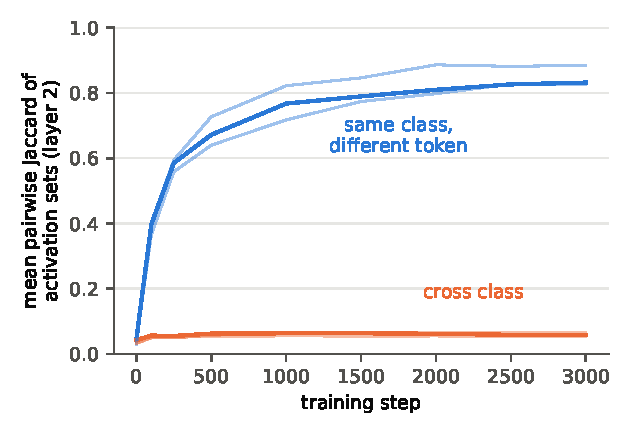
\includegraphics[width=0.62\linewidth]{figures/fig_emergence.pdf}
\caption{Raw activation-set similarity (registry-independent) on the synthetic
language, layer~2, three seeds (thin lines: seeds 1--2; thick: seed 0).
Same-class different-token similarity rises from chance-level (0.03--0.045,
equal to cross-class) to 0.83--0.89, while cross-class stays flat. The class
structure is created by training; the untrained network has none.}
\label{fig:emergence}
\end{figure}

\paragraph{Results (3 seeds).} Raw same-class Jaccard rises 0.03--0.045
$\rightarrow$ 0.826--0.885 while cross-class stays at 0.054--0.064
(Figure~\ref{fig:emergence}). The snapshot registry forms \emph{exactly 8
groups for 8 classes} in all three seeds with NMI(group, class) $=1.000$ at
coverage 1.00; NMI(group, token) is 0.694, matching the value computed for this
vocabulary's frequency profile (0.696) for groups that encode the class and
nothing else---i.e.\ the
groups are class abstractions, not token detectors (the token-detector
confound would show 64 groups and token-NMI 1.0; the untrained network is in
exactly that regime). The online registry ends with every used group at 100\%
class purity and zero cross-class pair merges, and stays structurally frozen
over 12{,}800 further inference-stream registrations (0 capacity merges, all
seeds). A layer contrast is consistent across seeds: layer~1 sets are
token-identity-dominated and churn ($\sim$30\% merge rate); layer~2 is where
class abstraction lives. \emph{Verdict: the first premise of the proposal is
true, cleanly, in the controlled setting.}

\section{Real text: emergence with a capacity law}
\label{sec:realtext}

On 4\,MB of real English (docstring prose; domain noted as a limitation), a
character-level model (vocab 96, seq 128) trains far past bigram statistics
(loss 1.33 vs.\ bigram 2.65). After training, same-character set similarity
\emph{falls} (0.82 $\rightarrow$ 0.13): real-language states are heavily
contextual, so the token-detector structure of the untrained net dissolves
into finer context states.

\begin{figure}[t]
\centering
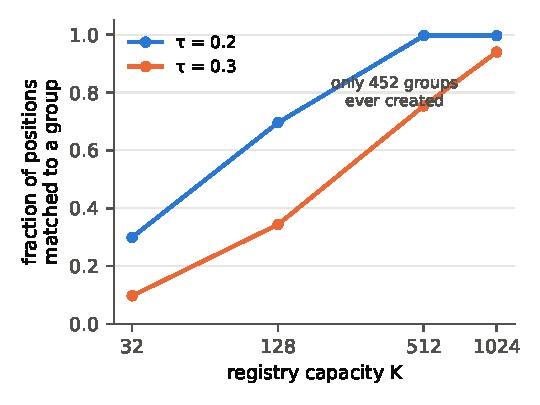
\includegraphics[width=0.5\linewidth]{figures/fig_realtext_capacity.pdf}
\caption{Real text: fraction of positions matched to some group as registry
capacity grows (frozen model, snapshot registries). At $K{=}512$,
$\tau{=}0.2$, coverage is 100\% with only $\sim$330--460 groups actually
opened: the states do organize into discrete assemblies, but the inventory is
hundreds, not the 8 of the planted-class setting.}
\label{fig:capacity}
\end{figure}

With the original $K{=}16$--$32$ the registry covers only 7--8\% of positions
(the one large stable group is the whitespace state). But a capacity sweep
(Figure~\ref{fig:capacity}) shows coverage 0.997 at $K{=}512$ with only
452 groups actually created (337 at a stricter set threshold)---the states
\emph{do} organize into a discrete inventory, sized in the hundreds for this
model, and raising $K$ to 1024 creates no further groups. Groups are finer
than characters (452 $\gg$ 96, NMI 0.60 to character identity) and align only
weakly with coarse human categories (NMI 0.24 to letter/digit/space/punctuation
classes): the model's
natural taxonomy is ``character $\times$ context state,'' not ours. We note,
without claiming equivalence, that this inventory size lands in the range
where sparse-autoencoder dictionaries operate for comparable models.
\emph{Verdict: emergence transfers to real language; the free parameter that
must scale is the assembly inventory.}

\section{Completion I: causal, content-specific, and it repairs in-site damage}
\label{sec:repair}

\paragraph{No deficit, no effect---and the placebo asymmetry.} On the
synthetic task, matching is essentially perfect at deployment (hit rate 1.0,
mean $\rrho$ 0.90) but completion changes nothing ($\Delta$loss
$\approx$ 0.0000): only 0.7 units per hit are missing, because even rare-ish
tokens (150--380 occurrences) are fully learned here. The decisive control:
\emph{placebo} injection of a wrong group's content at identical magnitude
degrades loss immediately (+0.019 at $\alpha{=}0.5$, +0.077 at
$\alpha{=}1.0$). The pathway is live; there was simply nothing to fix. This
placebo asymmetry---right content $\approx$ inert when nothing is missing,
wrong content always harmful---replicates in every subsequent experiment,
including during training (Section~\ref{sec:rare}), and is our standing
evidence that measured nulls are not dead-wire artifacts.

\begin{figure}[t]
\centering
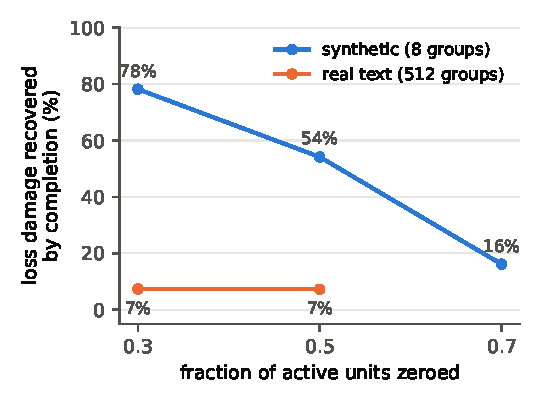
\includegraphics[width=0.5\linewidth]{figures/fig_repair.pdf}
\caption{Pattern completion repairs damage inflicted at its own site, and the
effect dilutes with assembly-inventory size. Synthetic task: 78/54/16\% of
corruption loss recovered at 30/50/70\% unit deletion, tracking the hit rate
(0.97/0.78/0.32) as corrupted cues fall below the match threshold. Real text
($K{=}512$, saturated at 512 groups): 7\% at both tested severities.}
\label{fig:repair}
\end{figure}

\paragraph{Partial cue $\rightarrow$ whole assembly, demonstrated.} When we
\emph{create} a deficit by zeroing a random 30/50/70\% of each position's
active units at the completion layer (corruption masks identical across
compared modes), completion recovers 78/54/16\% of the corruption-induced loss
(Figure~\ref{fig:repair}); placebo worsens it further. Recovery tracks the hit
rate: by 70\% deletion most corrupted cues no longer clear $\tau$, cleanly
localizing the retrieval failure point at $\rrho \approx \tau$. This is the
core assembly operation---a partial cue igniting its stored
completion---verified causally, with content specificity.

\paragraph{Dilution on real text.} Repeating the corruption protocol on the
real-text model with its $K{=}512$ registry recovers only 7\% at both drop 0.3
and 0.5, despite 93--96\% hit rates: matches occur at barely-threshold overlap
($\rrho \approx 0.34$) against fine-grained groups holding only $\sim$4
injectable units each, while the model's true dependence on these activations
is 100$\times$ larger than in the synthetic setting (corruption costs +0.23
vs.\ +0.002 nats). \emph{More groups $\Rightarrow$ less information per group
$\Rightarrow$ weaker completion}---the inventory size that emergence demands
(Section~\ref{sec:realtext}) is precisely what starves repair.

\section{Completion II: the rescue that fails, and why}
\label{sec:rare}

The motivating hope was to help \emph{naturally} under-trained inputs. We
engineered a stress regime: within-class token frequencies with an ultra-rare
tail (rank-7 tokens appear $\sim$77 times in training, rank-8 $\sim$11
times).

\paragraph{A statistical self-correction, reported as data.} Our first
estimate of the rare-token deficit (+0.126 nats) came from $n{=}130$ rare
positions without a standard error on the bucket difference. At $n{=}689$ the
deficit is $+0.060 \pm 0.043$---half the size and only marginally nonzero.
All paired comparisons in this paper carry paired SEs; we flag this because
several of our own intermediate conclusions had been framed against the
inflated number, and the correction materially changed the interpretation
that follows.

\paragraph{The deficit is embedding-rooted and fully repairable by an oracle.}
Replacing rare-token embeddings with their class-typical embedding (either the
class centroid or an actual frequent member) recovers the deficit completely
and precisely: paired $\Delta = -0.079 \pm 0.017$ on rare positions, residual
gap $\approx -0.02$. So a repair target exists and is reachable in principle.

\paragraph{Five mechanism variants all fail, for one measured reason.}
FFN-layer completion (single layer, multi-layer, embedding-layer with
absolute-value sets, two-pass cross-layer, and full-replacement variants)
recovers at most 11\% of the oracle bound. The account closes with one
measurement (Figure~\ref{fig:crossover}): correct-group retrieval for the
positions that need help is 99.4\% at 77 training occurrences but
\emph{52.0\%} at 11 ($n{=}1606$ and $230$ positions; chance is 12.5\%, and a
further 14\% of the rarest positions match no group at all, so only 44.8\% of
them are both matched and matched correctly). The complementary route is
closed too: those tokens' own embeddings identify their class only 25\% of the
time against a 12.5\% chance level, so a token cannot look up its own group
either. Since a wrong substitution costs on the order of $+1$ nat against an
available gain of $-$0.08, a $\sim$50\% error rate at the positions that need
help is not a discount on the benefit---it is a net loss an order of magnitude
larger than the benefit, and only the mechanism's timidity (it scales its pull
by the overlap $\rho$, which is low exactly where retrieval is unreliable)
keeps the measured effect near zero rather than strongly negative.
\emph{The tokens sick enough to need medicine are the tokens whose
prescription cannot be read.}

\begin{figure}[t]
\centering
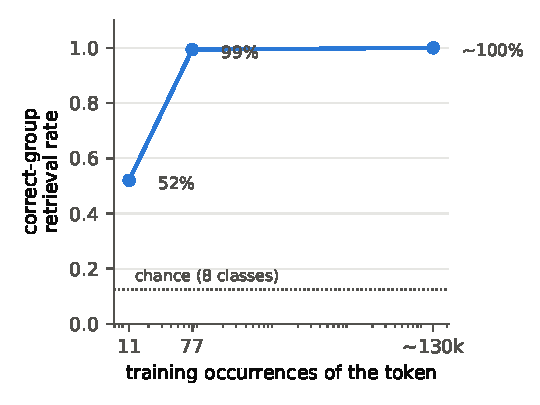
\includegraphics[width=0.48\linewidth]{figures/fig_crossover.pdf}
\caption{The need--reliability crossover. Correct-group retrieval (layer-2
sets, extreme-rarity model) collapses exactly for the tokens completion is
supposed to rescue. With wrong-content injection costing $\sim$10$\times$ the
available gain, a $\sim$50\% error rate at those positions cannot net a
benefit.}
\label{fig:crossover}
\end{figure}

\paragraph{In-training completion is safe but not self-organizing.} Running
registration \emph{and} completion inside the training loop (ramped in after
600 registration-only steps; 2 seeds $\times$ base, complete, placebo) neither
destabilizes training nor helps: overall loss is indistinguishable from
baseline (3.0975890 vs.\ 3.0976057 at seed 0, 3.0975857 vs.\ 3.0976009 at
seed 1---a difference of $1.6\times10^{-5}$ nats, which we report at full
precision because a rounded ``identical'' would be indistinguishable from a
silently disabled intervention), rare-token deltas are within noise, and switching
completion off at evaluation changes nothing---the model does not learn to
rely on the mechanism. The placebo arm is the informative one: persistent
wrong-content injection costs up to $+0.19$ loss while running, and
\emph{corrupts the model itself}---with the injection switched off at
evaluation the placebo-trained model is still $+0.064$ (seed 1) and $+0.044$
(seed 0) worse than baseline, so the damage is in the weights, not in the
intervention. Content specificity holds during learning, but the hoped-for
symbiosis does not arise in this task.

\section{Completion III: composition, and what the assemblies actually encode}
\label{sec:compose}

If assemblies capture reusable semantics, combining known assemblies should
answer novel combinations. We built a command language (64 primitives
$\times$ 4 repetition modifiers; answer = output token repeated 1--4 times)
where a coverage dial controls how many primitives each modifier is seen with.
The base model shows a clean composition dose--response on held-out
combinations: 2.4\% / 39.6\% / 88.5\% exact-match at coverage 8/16/32
primitives per modifier (test sets of 96--168 items; the pilot's 8--12-item
test sets and free memorization were redesigned away following a
pre-registered interpretation table). At the struggling tier (39.6\%),
completion moves nothing: 0 flips (L2), +2/144 (L1+L2, within noise), seen
combinations stay at 100\%, placebo flips 13 items to wrong.

The diagnostic explains it. Labelling every answer-region position two ways---by
which modifier produced it, and by how many outputs remain before EOS---and
scoring each registered group's purity against both labels separates the
hypotheses cleanly. The answer region's set-stable cores, registered either
during training or in a targeted post-hoc pass, organize by \emph{execution
progress}: the dominant group (112 of 149 covered positions, and the same
group under both archives) is ``one step left, about to emit EOS'' at
\textbf{1.00} purity \emph{across all modifiers}, while its purity against
modifier identity is 0.57 against a 0.44--0.51 chance level from the marginal.
The
composable ingredient the mechanism would need to inject is not what the
network's co-activation statistics stabilize. Injecting progress states
(the one structure that did form) also flips nothing. \emph{Verdict:
completion cannot add composition here, because ``what fires together'' is
the program counter, not the program.}

\section{The registry as a free internal-fault sentinel}
\label{sec:sentinel}

Every experiment above, success or failure, had one common feature: the
\emph{reading} $\rrho$ tracked state health precisely. That suggests
inverting the proposal---use the registry not to write into the stream but to
watch it.

\paragraph{Protocol.} Frozen real-text model; $K{=}512$ registry (built by
streaming registration, no labels, no fault examples); per-sequence
strangeness scores from the two readings of Section~\ref{sec:method}; AUC over
400 anomalous vs.\ 400 normal sequences (Hanley--McNeil SEs; two full
replications with different registry-construction and evaluation streams).

\begin{figure}[t]
\centering
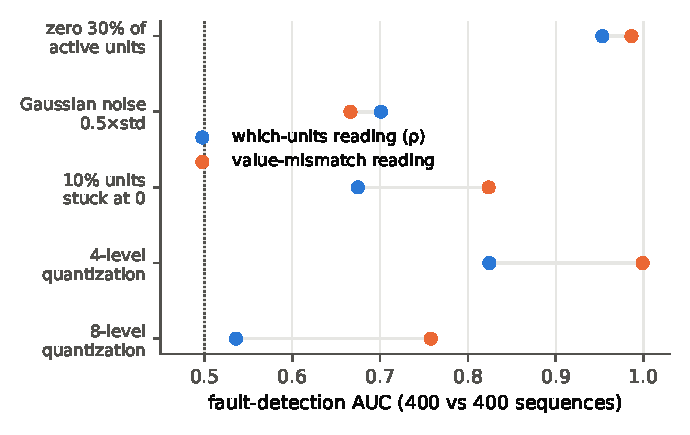
\includegraphics[width=0.6\linewidth]{figures/fig_sentinel.pdf}
\caption{Internal-fault detection by the two free readings (seed A shown;
seed B replicates within noise except 4-level quantization at 0.88). The
which-units reading owns topology faults (unit deletion); the value-mismatch
reading owns value faults (quantization) and dominates overall. Mild faults
(bottom rows' left points) remain hard.}
\label{fig:sentinel}
\end{figure}

\paragraph{Results.} \emph{Internal faults} (input normal, activations
damaged): moderate-severity faults of all four families are detected at AUC
0.95--1.00 by the better-suited reading (Figure~\ref{fig:sentinel}); mild
faults (10\% deletion, 0.5$\times$-std noise, 10\% stuck units) sit at
0.66--0.70 (low end 0.655). The value-mismatch channel closes most of the set-reading's
quantization blind spot (4-level: 0.82$\rightarrow$0.999; 8-level:
0.54$\rightarrow$0.76)---mechanistically the same lesson as completion's
failures: binary sets are blind to value distortions that preserve rank, so a
value channel is required. The residual 8-level case is a genuine limit: it
demonstrably harms the model ($+0.094$ nats) yet is only partially detected.
Measuring harm for every fault in the battery makes the more general point:
detection does not follow damage even here. Gaussian noise at $0.5\times$
costs $+0.295$ nats and is detected at 0.685, while 30\% unit deletion costs
less ($+0.227$) and is detected at 0.951. Section~\ref{sec:deploy} shows the
same dissociation on the 82M model, where it matters more.

\emph{Baseline.} The model's own per-sequence loss is the natural free rival.
On input-level anomalies (shuffled text, random tokens, case-shifted domain)
perplexity is at ceiling (1.000) and the registry readings are merely good
(0.976--1.000): output monitoring owns that regime and we claim nothing
there. On \emph{internal} faults the ranking reverses decisively: 0.955 vs.\
0.732 (30\% deletion), 0.996 vs.\ 0.856 (50\%). Output-level monitoring sees
a symptom; the registry palpates the site.

\begin{figure}[t]
\centering
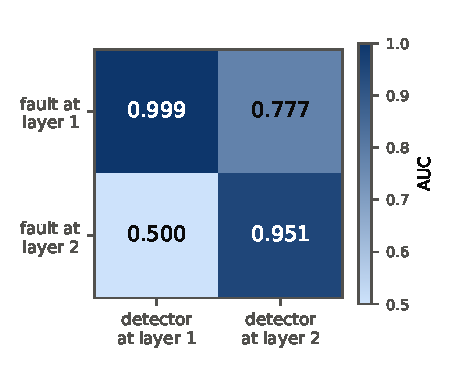
\includegraphics[width=0.42\linewidth]{figures/fig_localization.pdf}
\caption{Layer localization (both replications agree within 0.012). The
upstream detector is \emph{exactly at chance} when the fault is downstream---a
clean causal signature; damage propagates forward but attenuated. Rule: the
loudest (earliest) alarming layer is the fault site.}
\label{fig:localization}
\end{figure}

\emph{Localization.} Planting the fault at layer 1 vs.\ layer 2 and reading
both layers' registries yields the asymmetry of
Figure~\ref{fig:localization}: fault at L2 $\Rightarrow$ L1 detector at
0.500 (chance) and L2 at 0.95; fault at L1 $\Rightarrow$ L1 at 0.999, L2 at
0.78. Upstream silence identifies the site; no gradient, no profiling, no
second pass.

\paragraph{Honest position.} Activation-based runtime monitoring is an
established field (Section~\ref{sec:related}): distribution-fingerprint
monitors detect and localize inference-time silent corruptions at
$>$95\% \cite{drdna}; quantile monitors reach similar recall with
fault-injection-trained classifiers \cite{geissler}; binary activation
patterns \cite{cheng,olber} and box abstractions \cite{henzinger} monitor
novelty from offline-profiled patterns; Mahalanobis monitors need dataset
statistics \cite{lee}. Our claim is therefore \emph{not} that internal-fault
detection or localization is new. It is that (i)~the monitor here is a free
by-product of training---streaming registration, no post-hoc profiling pass,
no fault-injection calibration; (ii)~the dual which-units/value channels
dissociate fault families; (iii)~the upstream-silence signature localizes
without per-layer statistical modeling; and (iv)~the same structure supports
completion/repair, so monitoring and (in-site) repair share one mechanism.
Within our small-scale testbed these properties are demonstrated; their
survival at scale is untested (Section~\ref{sec:limits}).

\section{Scale-up: a real pretrained LM, and registration during real training}
\label{sec:realllm}

All results so far come from 34k--112k-parameter models trained by us. This
section reports the first transfer to a standard pretrained LM---distilgpt2
(82M parameters, 6 layers, 3072 FFN units per layer, run entirely on 2 CPU
cores)---including the configuration our own claim actually requires:
registration \emph{during} real gradient-based training.

\paragraph{Post-hoc deployment.} Streaming 4\,MB of English through the frozen
model builds registries ($K{=}2048$, $\tau{=}0.2$) on layers 2 and 4 in 74
seconds: layer~2 opens 1{,}999 groups, layer~4 only 175---the
deeper-layer-concentration pattern of Section~\ref{sec:emergence} replicates
on a real LM---with coverage 0.904/0.990. The fault battery (240 vs.\ 240
sequences) splits by fault type: \emph{unit-level} faults are detected
strongly (30\% unit deletion: 0.940; 30\% stuck-at-zero: 1.000), while
\emph{value-level} faults degrade relative to the toy setting (equal-magnitude
Gaussian noise: 0.576 vs.\ 0.97; 4-level quantization: 0.684 vs.\ 0.999). We
flag the value-fault degradation as unresolved; a plausible suspect is the
well-known outlier structure of GPT-2 activation magnitudes interacting with
our global scaling of injected distortions, but we did not run this down.
Localization is \emph{cleaner} than in the toy model: fault at layer 2
$\Rightarrow$ own detector 0.921 with the downstream echo at only 0.528;
fault at layer 4 $\Rightarrow$ upstream detector at exactly 0.500, own
detector 0.940.

\paragraph{Registration during real training.} An earlier draft of this
deployment stopped at the post-hoc pass above---which, as the project's
director pointed out, both departs from the original
register-while-pretraining design and contradicts our own
``no post-hoc profiling'' claim: profiling a frozen model post hoc is exactly
what existing monitors do. The missing experiment: continued pretraining of
distilgpt2 on the same corpus (400 AdamW steps, real weight updates; held-out
domain loss falls 4.084$\rightarrow$3.052), with the registry registering
inside the training forward passes. On the resulting model we compare three
archives under identical fault batteries:

\begin{center}
\small
\setlength{\tabcolsep}{4pt}
\begin{tabular}{@{}lcccc@{}}
\toprule
Archive & Coverage (L2/L4) & drop 30\% & stuck 30\% & quant-4 (value ch.) \\
\midrule
A: built during training & 0.70 / 0.99 & \textbf{0.935} & \textbf{1.000} & \textbf{0.969} \\
B: post-hoc on final model & 0.79 / 0.99 & 0.930 & 1.000 & --- \\
C: stale (pre-training archive) & 0.76 / 0.94 & 0.915 / \emph{0.591} & 1.000 / \emph{0.545} & --- \\
\bottomrule
\end{tabular}
\end{center}

\noindent (Archive A's localization matrix is intact: own layer 0.93--0.94,
upstream exactly 0.500. C's slashed pairs are which-units / value readings.)

Three findings. \emph{First}, the during-training archive matches the
post-hoc rebuild (A $\approx$ B, marginally better)---the free-by-product
property survives real weight drift, so the claim of
Section~\ref{sec:sentinel} now rests on the configuration it describes.
\emph{Second}, the during-training archive's value channel reaches 0.969 on
4-level quantization, largely repairing the post-hoc deployment's weakest
spot. \emph{Third}, the stale archive dissociates by channel (C row, slashed
numbers): the \emph{which-units} reading survives 400 steps of continued
training almost intact (0.915--1.000) while the \emph{value} reading
collapses (0.545--0.591). Co-activation topology is substantially more
persistent under training drift than activation magnitudes---an observation
with a practical corollary (only the value channel needs refreshing as a
model continues to train) and, we think, independent interest for the study
of what continued training actually changes.

\section{The sentinel at deployment scale: what it misses, and what it
false-alarms on}
\label{sec:deploy}

The AUC numbers of Sections~\ref{sec:sentinel}--\ref{sec:realllm} are
sequence-level separations measured on curated batches. Actually running the
monitor---one document at a time, deciding \emph{alarm} or \emph{no alarm}
without a matched control---exposed three things the AUCs hide. All results
here use the 82M model and the during-training archive, judging a document by
splitting it into 128-token blocks and alarming when more than 30\% of blocks
fall outside the calibrated range (150 documents of 2048 tokens per condition).

\paragraph{Three protocol defects found only by deployment.} \emph{(i)}~The
readings drift systematically with sequence length (layer 4: 0.887 at 16
tokens, 0.568 at 256), so a calibration taken at one length mis-scores another;
calibration must be length-binned. \emph{(ii)}~A single short text is not
judgeable---in-domain texts routinely reach $+1.9\sigma$ at shallow layers.
\emph{(iii)}~Judging a document by the \emph{mean} $z$ over its blocks fails
outright: the standard error shrinks as $1/\sqrt{n}$, so ordinary
paragraph-to-paragraph variation reads as many sigmas (a healthy model scores
$+4.6\sigma$). Counting the \emph{fraction of out-of-range blocks} is stable
where the mean is not. We report these because they are the difference between
a number in a table and a monitor that works.

\paragraph{Detection is not monotone in harm.} At 13\% in-domain false alarms:

\begin{center}
\small
\setlength{\tabcolsep}{5pt}
\begin{tabular}{@{}lccc@{}}
\toprule
Injected fault & Harm (nats) & Alarm rate & Correct layer \\
\midrule
L4, 30\% of active units deleted & $+0.046$ & \textbf{100\%} & 100\% \\
L4, 4-level quantization & $+0.718$ & \textbf{100\%} & 100\% \\
L2, 30\% of active units deleted & $+0.028$ & 99\% & 100\% \\
L4, 10\% of active units deleted & $+0.015$ & 71\% & 99\% \\
L4, 30\% of units stuck at zero & $+0.098$ & 54\% & 97\% \\
L4, 8-level quantization & $+0.258$ & 52\% & 95\% \\
L4, 10\% of units stuck at zero & $+0.029$ & 22\% & 87\% \\
L4, Gaussian noise $0.5\times$ & $+0.049$ & 20\% & 86\% \\
\bottomrule
\end{tabular}
\end{center}

Deleting 30\% of active units costs $+0.046$ nats and is caught every time;
freezing 30\% of units costs twice as much ($+0.098$) and is caught half the
time. What determines detection is whether the fault lands inside the
high-activation set the registry tracks, not how much damage it does. The
compensation is that \emph{localization is nearly free once an alarm fires}:
86--100\% of alarms name the correct layer across every fault type, including
the ones detected only half the time.

\paragraph{The blind spot, isolated.} We killed exactly 307 neurons (10\% of
the layer) three ways---only assembly members, only non-members, or at
random---and measured harm and alarm rate on the same 120 documents:

\begin{center}
\small
\setlength{\tabcolsep}{6pt}
\begin{tabular}{@{}lcc@{}}
\toprule
307 neurons killed & Harm (nats) & Alarm rate \\
\midrule
Healthy (no kill) & --- & 15\% \\
Members only (1300 available) & $+0.188$ & \textbf{75\%} \\
Non-members only (1772 available) & $+0.015$ & \textbf{15\%} (= baseline) \\
At random & $+0.022$ & 17\% \\
\bottomrule
\end{tabular}
\end{center}

Damage outside the assemblies is \emph{structurally} invisible: the alarm rate
is the healthy baseline to the digit. Two things follow. The reassuring one:
the registry watches the units that matter---the same number of member neurons
does $13\times$ the damage of non-members, and $8\times$ the damage of a random
draw, so the mechanism's field of view is concentrated on the load-bearing
part of the layer. (Superlinearity is part of this: killing 307 members costs
$+0.188$ while a random 307, containing roughly 130 members, costs only
$+0.022$.) The unreassuring one: a realistic random fault is mostly outside the
field of view, and at 10\% of a layer it is caught 17\% of the time---barely
above the 15\% false-alarm floor. \textbf{An alarm is informative; silence is
not evidence of health.}

\paragraph{The worst defect, and its fix.} A healthy model reading
out-of-domain text false-alarms at 95\% (Section~\ref{sec:sentinel}'s protocol
at scale: 13\% in-domain, 20\% on a neighbouring domain, 95\% on a far one).
This is fatal for a deployed monitor and it has a direct cause---the archive
describes one domain's state distribution, so any other domain looks like
internal damage. Two independent remedies, measured separately and together
(smaller archive budget than the factory configuration, so absolute rates are
comparable within this table only):

\begin{center}
\small
\setlength{\tabcolsep}{5pt}
\begin{tabular}{@{}lcccc@{}}
\toprule
Configuration & In-dom.\ FA & Near FA & Far FA & Detection / localization \\
\midrule
Single-domain archive & 32\% & 25\% & \textbf{99\%} & 100\% / 94\% \\
Multi-domain archive & 34\% & 5\% & 1\% & 100\% / 96\% \\
Within-document relative judging & \textbf{10\%} & 6\% & 97\% & 98\% / 98\% \\
\textbf{Both} & 17\% & \textbf{0\%} & \textbf{0\%} & \textbf{100\% / 100\%} \\
\bottomrule
\end{tabular}
\end{center}

Building the archive over three domains removes the out-of-domain false alarms
almost entirely; relative judging removes in-domain ones; together they retain
both benefits and cost nothing in detection or localization. A rule we had
proposed from single-document observation---that internal faults show as
\emph{one} layer alarming while domain mismatch shows as \emph{all} layers
alarming---did not survive this evaluation: out-of-domain text mostly triggers
the ``one layer'' pattern (91\% of its false alarms), so the pattern does not
separate the two causes and we withdraw it. A domain-diverse archive does the
job that the heuristic did not.

\section{Related work}
\label{sec:related}

\paragraph{Assemblies, fast weights, associative memory.} Assembly Calculus
formalizes cell-assembly operations in a dedicated random-graph model
\cite{papadimitriou}; Engram Neural Networks add differentiable Hebbian memory
with sparse retrieval to RNNs \cite{enn}; Plastic Transformers add
within-sequence Hebbian fast weights \cite{plastic}; modern Hopfield theory
identifies attention with pattern completion over continuous stored patterns
\cite{ramsauer}. Our registry differs in being a discrete, enumerable,
online-registered set structure bolted onto a standard Transformer, with
completion as explicit missing-member injection; our contribution relative to
this line is not architectural novelty but the measured map of where the
completion story does and does not cash out. Neuron co-activation has also
been registered for systems purposes (flash-memory layout) without any
completion semantics \cite{neuralink}. Sparse autoencoders recover
feature dictionaries whose size scales like our real-text inventory
\cite{sae}; they are offline analysis tools, where the registry is a runtime
mechanism---but the convergent inventory sizes are suggestive.

\paragraph{Runtime monitoring and fault detection.} Feature-space OOD
detection with class-conditional Gaussians \cite{lee}; abstraction/box
monitors \cite{henzinger} and their Gaussian variants; binary
neuron-activation-pattern monitors \cite{cheng,olber}; value-range clipping
against soft errors \cite{ranger}; quantile-feature fault detectors trained
on injected faults \cite{geissler}; and activation-distribution fingerprints
for detecting, localizing and mitigating silent data corruption
\cite{drdna}. We inherit this field's motivation and add the properties
listed at the end of Section~\ref{sec:sentinel}; we do not claim superiority
over tuned, profiled monitors, and a head-to-head at matched engineering
effort is future work.

\section{The carrier, not the idea: stored transformations succeed where stored
states fail}
\label{sec:transform}

Sections~\ref{sec:repair}--\ref{sec:compose} establish that stored \emph{states}
cannot be reused. This section reports the experiments that isolate \emph{why},
and the one substitution that turns the entire negative result positive.

\paragraph{States are context-bound; the failure is not about the injection
form.} Standard activation patching---replacing a deficient position's hidden
state with a donor's complete state---was never tested in the experiments above;
every intervention there was additive. Running the comparison properly
(Table~\ref{tab:patch}, $n{=}689$ rare positions) separates the two:

\begin{center}
\small
\begin{tabular}{@{}lcc@{}}
\toprule
Intervention at layer 2 & rare-token $\Delta$ & \% of oracle \\
\midrule
Replace with a real, \emph{same-context} donor state & $-0.0783 \pm 0.0153$ & 98\% \\
Replace with the registry's mean state (matched positions only) & $-0.0067 \pm 0.0093$ & n.s. \\
Add the stored typical values (the form used above) & $-0.0043 \pm 0.0020$ & 5\% \\
Oracle (embedding substitution) & $-0.0801 \pm 0.0166$ & 100\% \\
\bottomrule
\end{tabular}
\end{center}
\label{tab:patch}

An interpolation sweep, $h \leftarrow h + \lambda(\text{donor} - h)$, then rules
out ``increments are an illegitimate channel'' as the explanation: the benefit
rises smoothly and concavely with $\lambda$ (23\%, 51\%, 81\%, 95\%, 100\% of
the bound at $\lambda = 0.1, 0.25, 0.5, 0.75, 1.0$). Increments work fine---
provided they point at a genuine state. What fails is the \emph{content}, not
the arithmetic.

\paragraph{What counts as a legitimate state is narrower than ``real''.}
Substituting states of varying provenance (same sweep, same positions):

\begin{center}
\small
\begin{tabular}{@{}lc@{}}
\toprule
Substituted state & rare-token $\Delta$ \\
\midrule
Same class, \emph{same context} (donor) & $-0.0783$ \\
Same class, real, but from \emph{another sequence} & $+0.9152$ \\
Average of two real states & $+0.1356$ \\
Registry's cross-context mean (all positions) & $-0.0138$ (n.s.) \\
\bottomrule
\end{tabular}
\end{center}

A real state of the right class, transported from a different context, is
catastrophic---an order of magnitude worse than doing nothing. Averaging over
many contexts washes out the context-specific component and lands on something
inert; averaging two retains enough of the wrong context to do harm. A direct
remedy for the ``averaging destroys it'' hypothesis---storing 16 real exemplars
per group and substituting the nearest---recovers nothing
($-0.0037 \pm 0.0092$), because exemplars are themselves other-context states.
\emph{There is no stored state that is both reusable and informative.}

\begin{figure}[t]
\centering
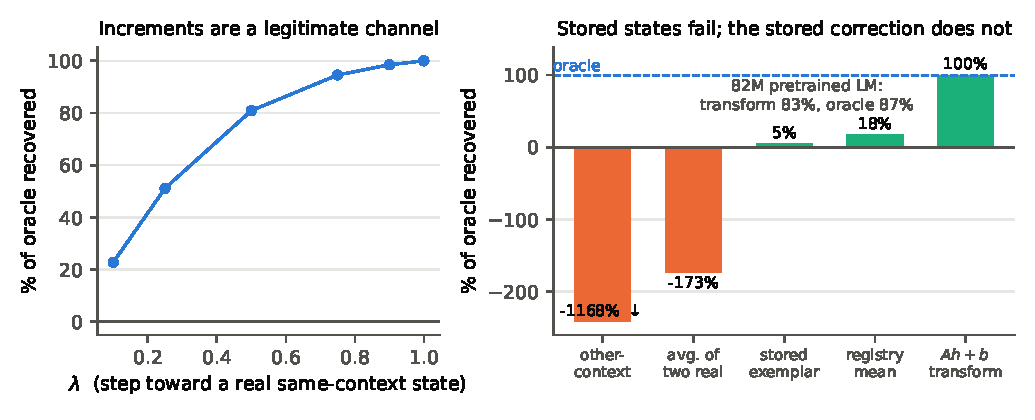
\includegraphics[width=\textwidth]{figures/fig_carrier.pdf}
\caption{The carrier, not the idea. \textbf{Left:} stepping a deficient state
toward a real same-context state recovers benefit smoothly and concavely with
step size---additive intervention is a legitimate channel, so the earlier
mechanism's additive form is not what broke it. \textbf{Right:} what breaks it
is \emph{what} is stored. Every stored \emph{state} fails---a real state of the
right class from another context is catastrophic (off scale), averages are
inert---while a single global linear \emph{correction} $Ah+b$, fit on one set
of contexts and applied to disjoint ones, recovers essentially all of the
oracle's benefit, and 95\% of it on an 82M pretrained model. Bars are \% of
the oracle intervention, $n{=}689$ rare positions.}
\label{fig:carrier}
\end{figure}

\paragraph{The correction, unlike the state, is context-free.} If states cannot
be transported, what can? We fit a linear map on (deficient state, correct
state) pairs from one set of contexts and evaluate on a disjoint set. Fitting
therefore requires a supervision signal---a healthy reference forward pass that
supplies the correct state---which the registry itself does not provide; what
the experiment establishes is that \emph{such a map exists and generalizes
across contexts}, not that it can be obtained without a teacher. Fitting is by
ridge regression on accumulated $X^\top X$ and $X^\top Y$, so it is a streaming
operation once the pairs are available.

\begin{center}
\small
\begin{tabular}{@{}lcc@{}}
\toprule
Stored object & synthetic ($n{=}689$) & real LM (82M, recovery) \\
\midrule
\textbf{Global linear map} $A h + b$ & $\mathbf{-0.0782 \pm 0.0153}$ (\textbf{99.9\%}) & \textbf{83\%} \\
Per-group maps $A_g h + b_g$ & $-0.0541 \pm 0.0123$ (69\%) & --- \\
Bias only $h + b$ (the original form) & $+0.0655 \pm 0.0146$ (harmful) & $-40\%$ \\
Stored mean state & --- & $-246\%$ \\
Oracle & $-0.0783 \pm 0.0153$ & 87\% \\
\bottomrule
\end{tabular}
\end{center}

A single global map recovers essentially all of the achievable benefit on
held-out contexts, and reaches 95\% of the oracle's recovery (83/87) on
distilgpt2. The bias-only variant---exactly the additive form the registry used
throughout Sections~\ref{sec:repair}--\ref{sec:compose}---is harmful at both
scales. Notably, conditioning the map on the registry's group assignment makes
it \emph{worse} (69\% vs.\ 99.9\%): the correction needs no retrieval at all.

\paragraph{Scope of the operator.} The map is specific to a damage type and a
data domain. Fit on 30\% unit deletion in-domain, it recovers 83\% there, 68\%
at a milder severity of the same damage and 77\% on a neighbouring domain, but
only 33\% (stuck units), 21\% (4-level quantization), and $-10\%$ (Gaussian
noise) across damage types, and $-9\%$ on a far domain---applying the wrong
operator actively harms, the same asymmetry seen with wrong-content injection
throughout. Fitting one map on a mixture of five damage types across three
domains buys coverage at the cost of peak accuracy: 59/-2/66/89/56\% across the
five damages (mean 54\% vs.\ 39\% for the specialized map applied to all five),
and a uniform 53--58\% across domains including the far one where the
specialized map was harmful. The single failure of the mixed operator---$-2\%$
on the \emph{mildest} damage---is over-correction: it applies an
average-severity correction where little is needed. That failure mode is
directly addressable with the severity estimate the sentinel of
Section~\ref{sec:sentinel} already produces for free, closing the loop between
detection and correction; we did not test it.

\paragraph{Reading.} The mechanism's headline failure was never about memory as
an idea. It was about the carrier. A network's states are context-bound and
cannot be stored and replayed; the map from a deficient state to the correct one
is context-free and can be. This single substitution converts the null result of
Sections~\ref{sec:repair}--\ref{sec:compose} into a positive one, and it does so
without retrieval, without grouping, and without any component of the registry
except the pairs used to fit it.

\section{Limitations}
\label{sec:limits}

Scale: the mechanistic dissection uses 34k--112k-parameter models, and the
sentinel is additionally validated on an 82M pretrained LM
(Section~\ref{sec:realllm})---but 82M is still small, the continued
pretraining was 400 steps on one domain, and nothing is demonstrated for
production-scale models; several phenomena (inventory size, dilution, the
need--reliability crossover, the value-fault degradation) plausibly sharpen
with scale in unknown directions. Data: one synthetic family, one command
language, and
4\,MB of technical-domain English; the real-text results should be read as
``real language at character level in one domain.'' Design space: thresholds
($\tau$, the 50\%-of-max rule, EMA rates) were fixed early and swept only
where reported (capacity $K$; $\tau \in \{0.2, 0.3\}$); the sentinel's mild-fault
regime (AUC $\approx$ 0.7) and residual fine-quantization gap (0.76) are open;
sequence-level scores were position means, and better aggregation is likely
easy headroom. The in-training completion loop used conservative
registration-before-injection ordering; feedback variants (registering
post-injection states) are untested. The correction operator of
Section~\ref{sec:transform} is the paper's one positive transfer result and
carries its own three limits: it is fit under supervision from a healthy
reference pass, so we show that a context-free correction \emph{exists}, not
that a network can discover one unaided; it is scope-bound to a damage type and
domain, and misapplication harms; and the linear family is the simplest one we
tried, not a searched choice. Finally, our fault families are
synthetic injections; real hardware / compression faults have structure we
did not model.

\section{Conclusion}

We took a bio-inspired proposal seriously enough to measure every link of its
chain, and the map that resulted has three parts.

The foundation holds. Co-activation assemblies emerge during ordinary training,
are captured online for free, and their content is causally live---injections
help when damage sits at the injection site and reliably hurt when the content
is wrong, in every experiment we ran.

The proposal's own mechanism fails, and we can say exactly why. Not because
memory is the wrong idea, but because a stored \emph{state} is the wrong
carrier. Network states are context-bound: a real state of the right class,
moved from another context, is an order of magnitude worse than doing nothing;
averaged states are inert; stored exemplars are no better. Every downstream
failure follows from this---the tokens needing completion cannot be retrieved
reliably, the stable co-activation cores encode execution progress rather than
composable semantics, and repair dilutes as the assembly inventory grows.

The substitution that works is small and total. The map from a deficient state
to the correct one is context-free where the states are not: a single global
linear operator, fit on one set of contexts and applied to disjoint ones,
recovers 99.9\% of the achievable benefit in the synthetic setting and 95\% of
the oracle's recovery on a real 82M model---while the additive form the original
mechanism used is harmful at both scales, and conditioning on the registry's
groups makes it worse. The operator is specific to a damage type and a data
domain, and applying the wrong one harms; a mixed-fit operator trades peak
accuracy for uniform coverage.

And the registry's readings, which no longer serve retrieval, turn out to be a
zero-calibration, streaming, layer-localizing internal-fault sentinel that
complements output-level monitoring exactly where the latter is blind. Run as a
monitor rather than scored as a classifier, it earns a sharper description:
its alarms are trustworthy and almost always name the right layer, its silence
is not evidence of health---damage outside the assemblies is invisible by
construction---and it is only usable outside its archive's domain if the
archive was built across domains, which costs nothing and fixes a 95\% false-alarm
rate outright.

One mechanism, honestly mapped: a poor librarian of states, a competent teacher
of corrections, and a good witness to damage.

\begin{thebibliography}{9}
\small
\bibitem{papadimitriou} C.~H. Papadimitriou, S.~S. Vempala, D.~Mitropolsky,
M.~Collins, W.~Maass. Brain computation by assemblies of neurons.
\emph{PNAS} 117(25), 2020.
\bibitem{enn} Engram Neural Networks: Hebbian memory with sparse attention
retrieval. arXiv:2507.21474, 2025.
\bibitem{plastic} Plastic Transformers: Hebbian and gradient plasticity as
fast weights. arXiv:2510.21908, 2025.
\bibitem{ramsauer} H.~Ramsauer et al. Hopfield networks is all you need.
\emph{ICLR}, 2021.
\bibitem{neuralink} Neuralink: Neuron co-activation linking for efficient
LLM inference on flash. arXiv:2410.19274, 2024.
\bibitem{sae} T.~Bricken et al. Towards monosemanticity: decomposing language
models with dictionary learning. Anthropic, 2023; and successors.
\bibitem{lee} K.~Lee, K.~Lee, H.~Lee, J.~Shin. A simple unified framework for
detecting out-of-distribution samples and adversarial attacks.
\emph{NeurIPS}, 2018.
\bibitem{cheng} C.-H. Cheng, G.~N\"uhrenberg, H.~Yasuoka. Runtime monitoring
neuron activation patterns. \emph{DATE}, 2019.
\bibitem{henzinger} T.~A. Henzinger, A.~Lukina, C.~Schilling. Outside the
box: abstraction-based monitoring of neural networks. \emph{ECAI}, 2020.
\bibitem{olber} B.~Olber et al. Detection of out-of-distribution samples
using binary neuron activation patterns. \emph{CVPR}, 2023.
\bibitem{ranger} Z.~Chen, G.~Li, K.~Pattabiraman. Ranger: boosting error
resilience of deep neural networks through range restriction. \emph{DSN},
2021.
\bibitem{geissler} F.~Geissler et al. Activation-based runtime fault
detection for safety-critical DNNs. 2023. arXiv:2310.20349.
\bibitem{drdna} F.~Ma et al. Dr.~DNA: combating silent data corruption in
deep learning using distribution of neuron activations. \emph{ASPLOS}, 2024.
\end{thebibliography}

\end{document}
